\section{Ziel}

\section{Theorie}
\label{sec:Theorie}

\subsection{Aufbau und Wirkungsweise eines Geiger-Müller-Zählrohrs}

Das Zählrohr besteht wie in Abb. \ref{fig:zaehlrohr} zu erkennen aus einem Kathodenzylinder mit Radius $r_\text{k}$ und einem Anodendraht mit Radius $r_\text{a}$. Im Inneren befindet sich ein Gasgemisch. Indem an das Äußere des Rohrs und den Draht eine äußere Spannung angelegt wird, entsteht ein radiales E-Feld. Die Feldstärke beträgt 
\begin{equation*}
    E(r) = \frac{U}{r ln(\frac{r_\text{k}}{r_\text{a}})}.
    \label{eqn:feldstärke}
\end{equation*}

Die Beschleunigung des Teilchens kann somit beliebig groß werden, wenn der Radius des Drahtes beliebig klein gewählt wird. %wichtig?

\begin{figure}
    \centering
    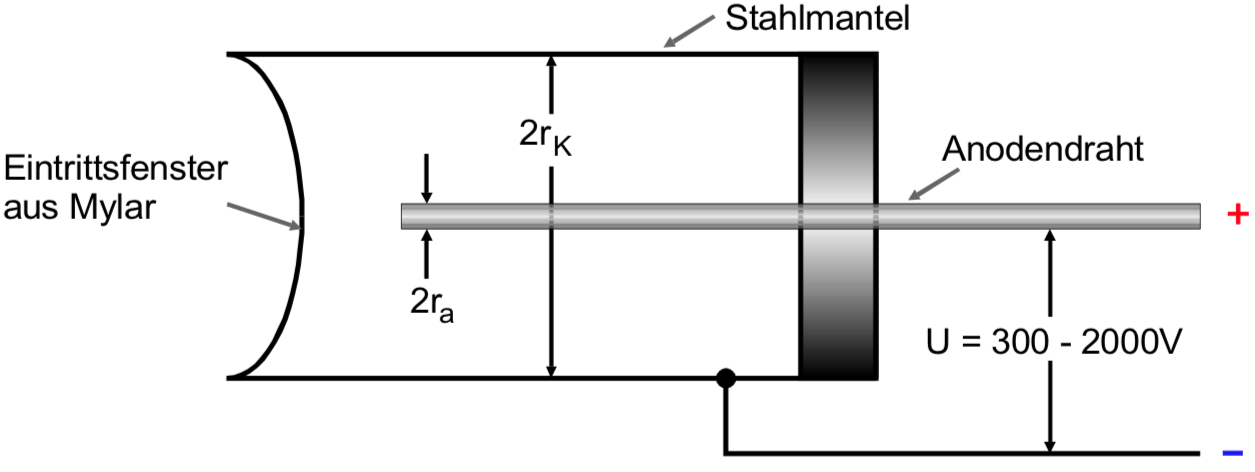
\includegraphics[width=12cm, height=8cm]{build/zaehlrohr.png}
    \caption{Zu sehen ist der Aufbau eines Geiger-Müller-Zählrohrs. Der äußere Zylinder ist die Kathode und der Draht die Anode. Das Eintrittsfenster besteht aus einer durch den Druck nach innen gewölbten Mylar-Folie. \cite{V703}}
    \label{fig:zaehlrohr}
\end{figure}

%Bereich II
Durch die Energie des eindringenden Teilchens werden Atome ionisiert und Elektronen werden losgelöst. Je nach angelegter Spannung können dann verschiedene Phänomene auftreten. Ein Gerät, das nur so viel Spannung benutzt, dass der Ionisationsstrom proportional zur Energie und Intensität der einfallenden Strahlung ist, ist eine Vorstufe zum Zählrohr und wird Ionisationskammer genannt. 

%Bereich III
Wenn die Energie der Elektronen groß genug ist, um ihrerseits Atome zu ionisieren, wird dieser Vorgang Stoßionisierung genannt. Wenn lawinenartig die Zahl der freien Elektronen zunimmt, wird dies eine Townsend-Lawine genannt. 
Die Ladung ist dann so groß, dass sie als Ladungsimpuls gemessen werden kann.
Eine Proportionalität zwischen der Ladung $Q$ und der Primärteilchenenergie definiert das Zahlrohr dann als Proportionalitätzählrohr. 

%Bereich IV
Sobald der Proportionalitätsbereich überschritten ist, wird der Auslösebereich erreicht, der eigentliche Arbeitsbereich des Geiger-Müller-Zählrohrs. Die dabei entstehenden UV-Photonen können sich auch senkrecht zu den Feldlinien bewegen und so auch an anderen Stellen noch zusätzliche Elektronen loslösen. So entstehen im gesamten Zählrohr weitere Lawinen. 

\subsection{Totzeit, Nachentladung}
%Totzeit
Während die Elektronen schnell zum Draht wandern, bleiben die positiven Ionen aufgrund der größeren Masse länger im Gasraum. Sie bauen vorübergehend einen sogenannten "Ionenschlauch" auf. Für eine bestimmte Zeit sind dann keine Stoßionisationen mehr möglich, da die Feldstärke dadurch verringert wird. Diese Zeit wird Totzeit genannt, weil währenddessen kein Teilchen registriert werden kann. 
%Erholungszeit
Den Zeitraum, der sich anschließt, bis dies wieder funktioniert, wird Erholungszeit genannt. 
%Nachentladungen
Auf den Zählrohrmantel auftreffende Ionen können dort Elektronen aus der Oberfläche befreien. Diese "Sekundärelektronen" können die Zählrohrentladung erneut zünden, sodass durch den Durchgang nur eines Teilchens mehrere zeitlich versetzte Ausgangsimpulse entstehen können. 
Diese Impulse werden Nachentladungen genannt. 
Um diese Impulse zu verhindern, sind Gase im Inneren des Rohres vorhanden. Die Edelgasionen stoßen dann nämlich mit den Atomen den Gasmolekülen zusammen und ionisieren diese. Die haben dann aber weniger Energie und können somit nicht zu Nachentladungen führen. 


\subsection{Charakteristik des Zählrohrs}

Wenn die Teilchenzahl $N$ bei konstanter Strahlungsintensität gegen die angelegte Spannung $U$ aufgetragen wird, entsteht eine Charakteristik wie in Abb. \ref{fig:charakteristik}. Bei der Spannung $U_\text{E}$ setzt der Auslösebereich ein. Der darauf folgende lineare Teil wird Plateau genannt. Die Steigung des Plateaus sollte am besten null sein. Am Ende des Plateaus nimmt die Anzahl der Nachentladungen extrem zu. Sie geht über in den Bereich der selbstständigen Gasentladung, der sehr schädlich ist für ein Strahlrohr.

\begin{figure}
    \centering
    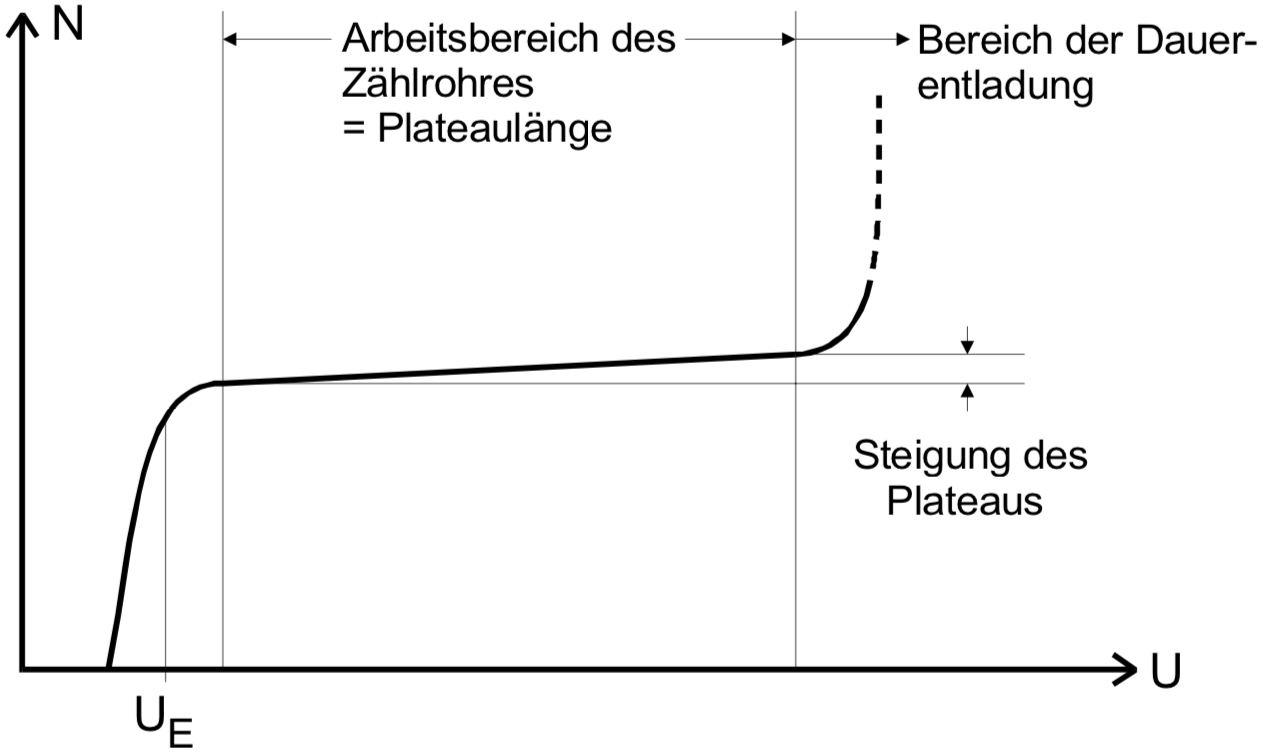
\includegraphics[width=12cm, height=8cm]{build/charakteristik.png}
    \caption{Es ist die Zählrohrcharakteristik zu sehen. Die Zählrate $N$ wird dabei gegen die angelegte Spannung $U$ aufgetragen. Durch die vertikalen Linien werden der Arbeitsbereich des Zählrohrs und der Bereich der Dauerentladung gekennzeichnet. Es ist außerdem die Steigung des Plateaus eingezeichnet. \cite{V703}}
    \label{fig:charakteristik}
\end{figure}

\subsection{Ansprechvermögen des Zählrohrs}

Das Ansprechvermögen ist die Wahrscheinlichkeit dafür, dass ein Teilchen im Zählrohr nachgewiesen wird. Für $\alpha$- und $\beta$-Teilchen liegt diese bei fast \SI{100}{\percent}. Wichtig ist, dass die Teilchen überhaupt in das Rohr gelangen. Es wird eine Mylar-Folie als Fenster verwendet. Diese Folie ist leicht nach innen gewölbt, durch den Unterdruck im Inneren des Rohres. %mit der Folie schon erwähnt